% UATD sonar detection: DEIM-D-FINE-S project update (comparison with RF-DETR-S and YOLO26n).
% Tables in generated/ and figures in figures/ are produced by
%   python scripts/make_report_assets.py --model deim ...   (do not edit them by hand)
% Yellow "Write this in your own words" boxes mark the text the students must write.
% Compile with pdfLaTeX (Overleaf default) or Tectonic.
\documentclass[11pt,a4paper]{article}

\usepackage[T1]{fontenc}
\usepackage[utf8]{inputenc}
\usepackage{lmodern}
\usepackage[margin=2.3cm,headheight=14pt]{geometry}
\usepackage{graphicx}
\usepackage{booktabs}
\usepackage{longtable}
\usepackage{array}
\usepackage{amsmath}
\usepackage{xcolor}
\usepackage{float}
\usepackage{caption}
\usepackage{fancyhdr}
\usepackage{titlesec}
\usepackage{enumitem}
\usepackage[most]{tcolorbox}
\usepackage{tikz}
\usetikzlibrary{positioning,arrows.meta,shapes.misc}
\usepackage[hidelinks]{hyperref}

\definecolor{accent}{HTML}{6A3D8F}
\definecolor{muted}{HTML}{6B7785}
\captionsetup{font=small,labelfont=bf}
\setlist{nosep}

\pagestyle{fancy}
\fancyhf{}
\fancyhead[L]{\small\color{muted}UATD / DEIM-D-FINE-S \textbullet{} Project Update}
\fancyhead[R]{\small\color{muted}\thepage}
\fancyfoot[L]{\scriptsize\color{muted}Numbers generated from run \texttt{dfine\_s\_s0} by the shared evaluator}
\renewcommand{\headrulewidth}{0.4pt}

\titleformat{\section}{\Large\bfseries\color{accent}}{\thesection}{0.8em}{}
\titleformat{\subsection}{\large\bfseries\color{accent}}{\thesubsection}{0.6em}{}

% Placeholder for text the students write themselves (CLAUDE.md rule 4).
\newtcolorbox{writehere}{enhanced,breakable,colback=yellow!8,colframe=orange!75!black,
  fonttitle=\bfseries\small,title={Write this in your own words},fontupper=\small}

\newcommand{\gentab}[1]{\input{generated/#1}}

\begin{document}

% ------------------------------------------------------------------ title page
\begin{titlepage}
\centering
\vspace*{1.5cm}
% \includegraphics[width=2.6cm]{figures/nsu_logo.png}\\[0.6cm]  % add the logo file to use it
{\Large\bfseries North South University}\\[2pt]
Department of Electrical \& Computer Engineering\\[1.4cm]
\rule{\linewidth}{0.4pt}\\[0.4cm]
{\Huge\bfseries Project Update}\\[0.3cm]
\rule{\linewidth}{0.4pt}\\[1.2cm]
{\LARGE\bfseries Underwater Sonar Object Detection:\\[4pt] DEIM-D-FINE-S compared with RF-DETR}\\[1.2cm]
\begin{tabular}{rl}
\textbf{Course} & CSE 499A, Section 12\\
\textbf{Supervisor} & Dr.\ Riasat Khan
\end{tabular}\\[1.4cm]
\begin{tabular}{lll}
\toprule
\textbf{Student Name} & \textbf{Student ID} & \textbf{Email}\\
\midrule
Walidur Rahman & 231 1712 642 & walidur.rahman01@northsouth.edu\\
Mridha Fahad Hossain & 231 2199 042 & mridha.hossain@northsouth.edu\\
Nafsin Nasama Salmee & 231 1776 642 & nafsin.salmee@northsouth.edu\\
Md.\ Azmine Amin Mormo & 231 2318 042 & azmine.mormo@northsouth.edu\\
\bottomrule
\end{tabular}\\[1.4cm]
\textbf{Submission Date:} \today
\end{titlepage}

\tableofcontents
\newpage

% ------------------------------------------------------------------ 1 overview
\section{Overview}
\subsection{Executive summary}
\begin{writehere}
Points to cover:
\begin{itemize}
  \item Second detector on the same fixed split and shared evaluator: DEIM (Huang et al., CVPR 2025) training method on the D-FINE detector (Peng et al., ICLR 2025), small model, fine-tuned from COCO weights.
  \item Role: comparison row. DEIM/D-FINE come from the RT-DETR codebase, which a classmate works on; RF-DETR stays the main pipeline.
  \item Why chosen: our RF-DETR results showed localisation as the main gap (test mAP75 0.26 / 0.25); D-FINE models box edges as probability distributions, DEIM adds more positive matches per image (UATD has 1--3 objects per image).
  \item Headline: test mAP50:95 0.376 / 0.383 (RF-DETR 0.368 / 0.363, YOLO26n 0.329 / 0.337); mAP75 0.290 / 0.286 (RF-DETR 0.261 / 0.246); mAP50 about equal (0.809 / 0.833 vs 0.815 / 0.825).
  \item Remaining problems: cube (AP50 0.61 on both tests), cage classes, tiny boxes on test1.
\end{itemize}
\end{writehere}

\begin{table}[H]\centering
\caption{Headline detection performance of DEIM-D-FINE-S (mAP at IoU 0.5).}
\gentab{tab_headline}
\end{table}

\begin{table}[H]\centering
\caption{All models on the same split. $^\dagger$YOLO26n values are copied from the original notebook (Ultralytics validator, input 640); RF-DETR-S (input 512) and DEIM-D-FINE-S (input 640) come from our shared evaluator (pycocotools + Ultralytics-definition P/R/F1). Best per split and column in bold.}
\label{tab:compare}
\gentab{tab_compare}
\end{table}

\subsection{Objectives}
\begin{writehere}
Points to cover: add a strong recent real-time DETR as a comparison row; keep everything else identical (split, val-only selection, effective batch 16, seed 0, shared evaluator); test whether a detector built for box precision closes the mAP75 gap; feed the comparison into the error analysis and the choice of the tiny-object method (roadmap steps 7--8).
\end{writehere}

% ------------------------------------------------------------------ 2 dataset
\section{Dataset}
The dataset, fixed split and cleaning are identical to the RF-DETR report.

\begin{table}[H]\centering
\caption{Images and objects per split after cleaning.}
\gentab{tab_dataset}
\end{table}

\begin{table}[H]\centering
\caption{Objects per class and split.}
\gentab{tab_class_counts}
\end{table}

\begin{figure}[H]\centering
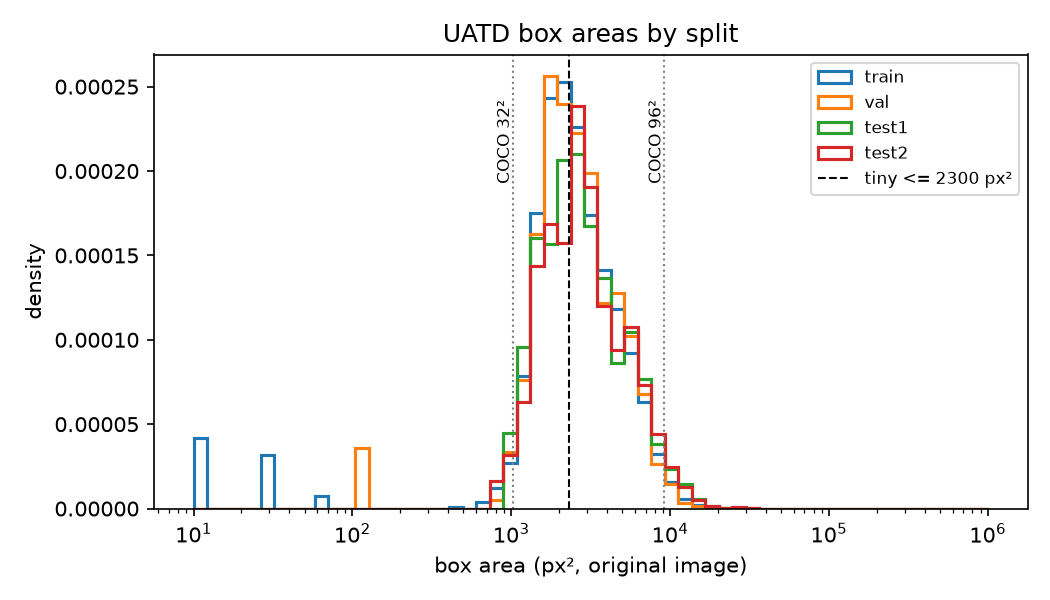
\includegraphics[width=0.49\linewidth]{figures/box_area_by_split.png}\hfill
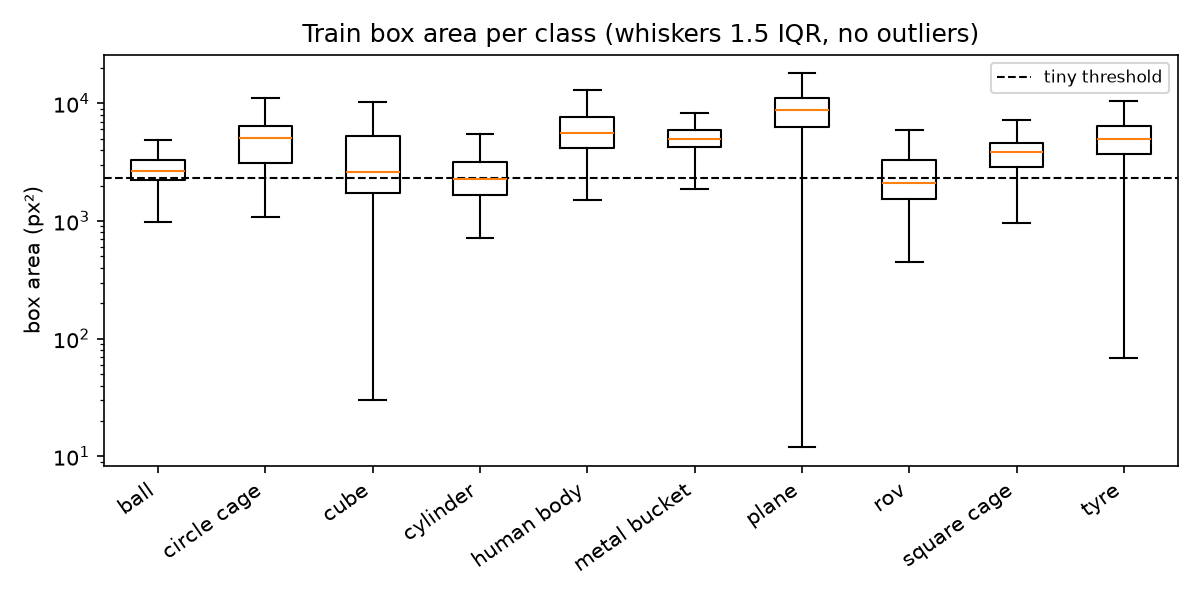
\includegraphics[width=0.49\linewidth]{figures/box_area_per_class_train.png}
\caption{Box area per split and per class (train). The dashed line marks the tiny threshold (2300\,px$^2$, the 25th percentile of train box areas), frozen before any model was evaluated.}
\end{figure}

% ------------------------------------------------------------------ 3 methodology
\section{Methodology}
\subsection{Pipeline}
\begin{figure}[H]\centering
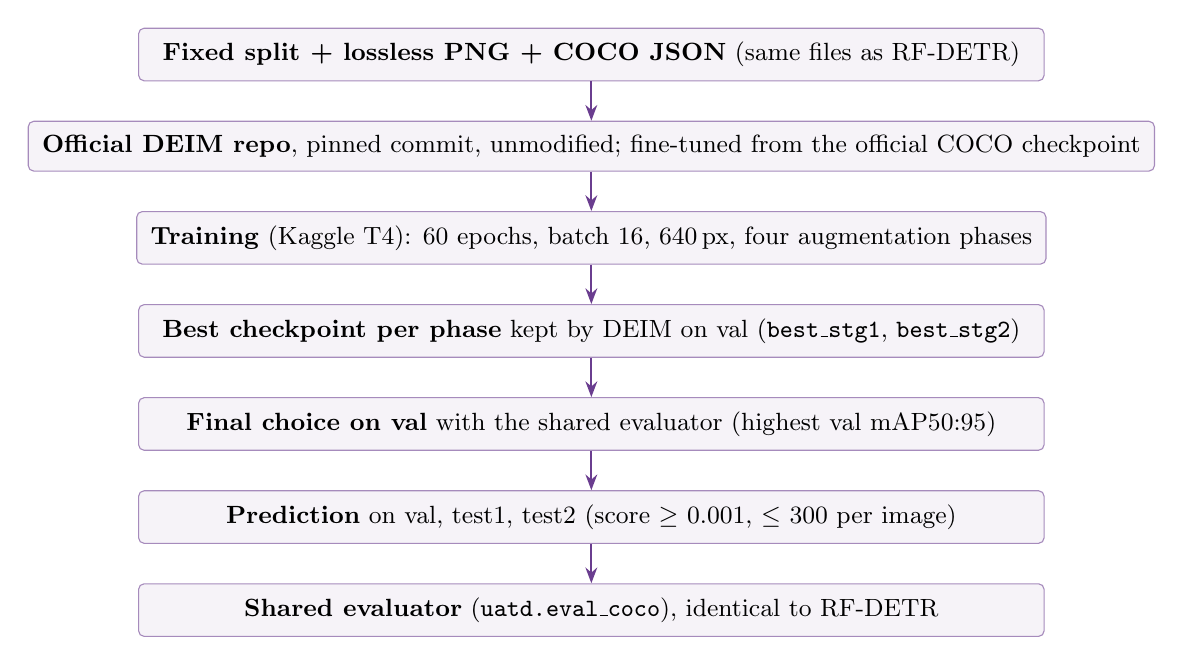
\begin{tikzpicture}[
  node distance=5mm,
  box/.style={draw=accent!60,fill=accent!6,rounded corners=2pt,minimum width=11.5cm,align=center,font=\small,inner sep=5pt},
  arr/.style={-{Stealth[length=2mm]},accent,thick}]
\node[box] (a) {\textbf{Fixed split + lossless PNG + COCO JSON} (same files as RF-DETR)};
\node[box,below=of a] (b) {\textbf{Official DEIM repo}, pinned commit, unmodified; fine-tuned from the official COCO checkpoint};
\node[box,below=of b] (c) {\textbf{Training} (Kaggle T4): 60 epochs, batch 16, 640\,px, four augmentation phases};
\node[box,below=of c] (d) {\textbf{Best checkpoint per phase} kept by DEIM on val (\texttt{best\_stg1}, \texttt{best\_stg2})};
\node[box,below=of d] (e) {\textbf{Final choice on val} with the shared evaluator (highest val mAP50:95)};
\node[box,below=of e] (f) {\textbf{Prediction} on val, test1, test2 (score $\geq$ 0.001, $\leq$ 300 per image)};
\node[box,below=of f] (g) {\textbf{Shared evaluator} (\texttt{uatd.eval\_coco}), identical to RF-DETR};
\foreach \u/\v in {a/b,b/c,c/d,d/e,e/f,f/g} \draw[arr] (\u) -- (\v);
\end{tikzpicture}
\caption{DEIM-D-FINE-S pipeline. Test1 and test2 enter only at the prediction step.}
\end{figure}

\subsection{DEIM-D-FINE}
\begin{writehere}
Points to cover (cite both papers):
\begin{itemize}
  \item D-FINE (ICLR 2025): real-time DETR; HGNetv2 CNN backbone, hybrid encoder, 3-layer decoder, 300 queries; predicts each box edge as a probability distribution over 32 bins and refines it layer by layer (Fine-grained Distribution Refinement, FGL loss); distils the last layer's localisation into earlier layers (GO-LSD, DDF loss).
  \item DEIM (CVPR 2025): Dense one-to-one matching (Mosaic + MixUp put more objects in each image, so more positive matches) and the Matchability-Aware Loss (MAL); designed for fast convergence.
  \item Set-based matching, so no NMS.
  \item Relation to RT-DETR: same codebase family (classmate's topic), so used only as a comparison row.
\end{itemize}
\end{writehere}

\begin{table}[H]\centering
\caption{DEIM-D-FINE-S configuration, read from the fully merged config that ran (official S config + \texttt{configs/deim/uatd\_deim\_dfine\_s.yml}).}
\gentab{tab_train_config}
\end{table}

\begin{writehere}
Points to cover on the settings we changed and why (all fixed before training, none tuned on test): 60-epoch recipe from the DEIM authors instead of 132 epochs (fine-tuning from COCO weights; 132 epochs $\approx$ 20 h on a T4); batch 16 instead of 32 to match RF-DETR, learning rates halved by the repo's linear rule; EMA and warm-up lengths kept the same in epochs as the official recipe (UATD epoch = 427 iterations vs 3697 on COCO), otherwise the EMA weights used for selection would average over $\sim$25--50 epochs.
\end{writehere}

\subsection{Evaluation protocol}
Identical to the RF-DETR report: pycocotools COCO metrics, Ultralytics-definition P/R/F1 (IoU 0.5, at the confidence of maximum mean F1 on each split), per-class AP, and AP on the frozen tiny / non-tiny bins.

% ------------------------------------------------------------------ 4 training
\section{Training}
\begin{table}[H]\centering
\caption{Execution environment and run summary.}
\gentab{tab_environment}
\end{table}

\begin{figure}[H]\centering
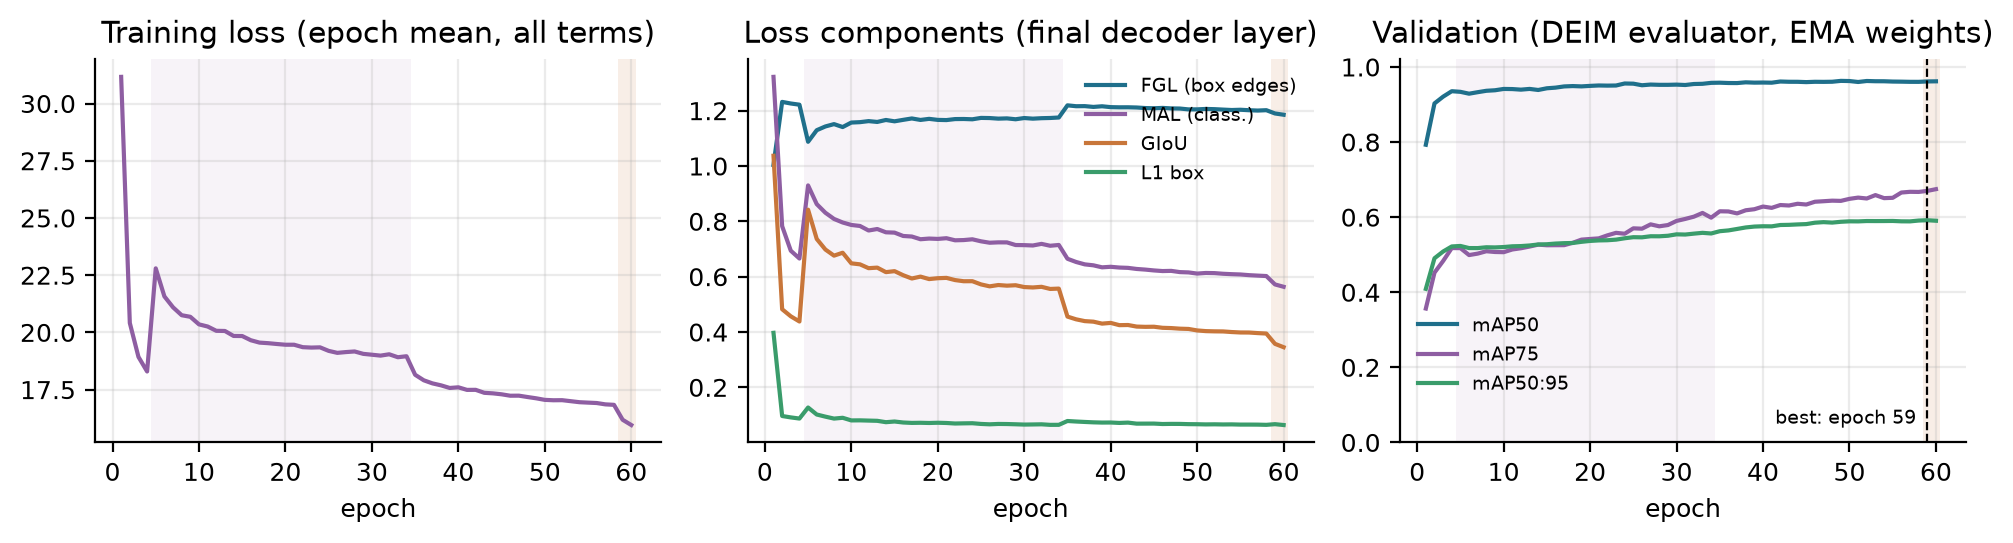
\includegraphics[width=\linewidth]{figures/fig_training_curves.png}
\caption{Training losses and validation metrics per epoch (DEIM's built-in evaluator on the EMA weights; used only for monitoring and checkpoint selection). Purple band: Mosaic + MixUp phase (epochs 5--34). Orange band: final no-augmentation phase (59--60). Dashed line: best val epoch.}
\end{figure}

\begin{writehere}
Points to cover: 60 epochs in 8.5\,h, one session; loss steps up at epoch 5 (Mosaic/MixUp start) and down at 35 (they stop) and 59 (augmentation stops); val mAP50:95 still rising slowly until the end (0.59), mAP75 rises most; best val epoch 59 (final phase), and \texttt{best\_stg2} also wins on val with the shared evaluator (0.592 vs 0.591); full log in Appendix~\ref{app:epochs}.
\end{writehere}

% ------------------------------------------------------------------ 5 evaluation
\section{Evaluation}
\subsection{Overall results}
\begin{table}[H]\centering
\caption{DEIM-D-FINE-S overall performance (shared evaluator).}
\gentab{tab_overall}
\end{table}

\begin{figure}[H]\centering
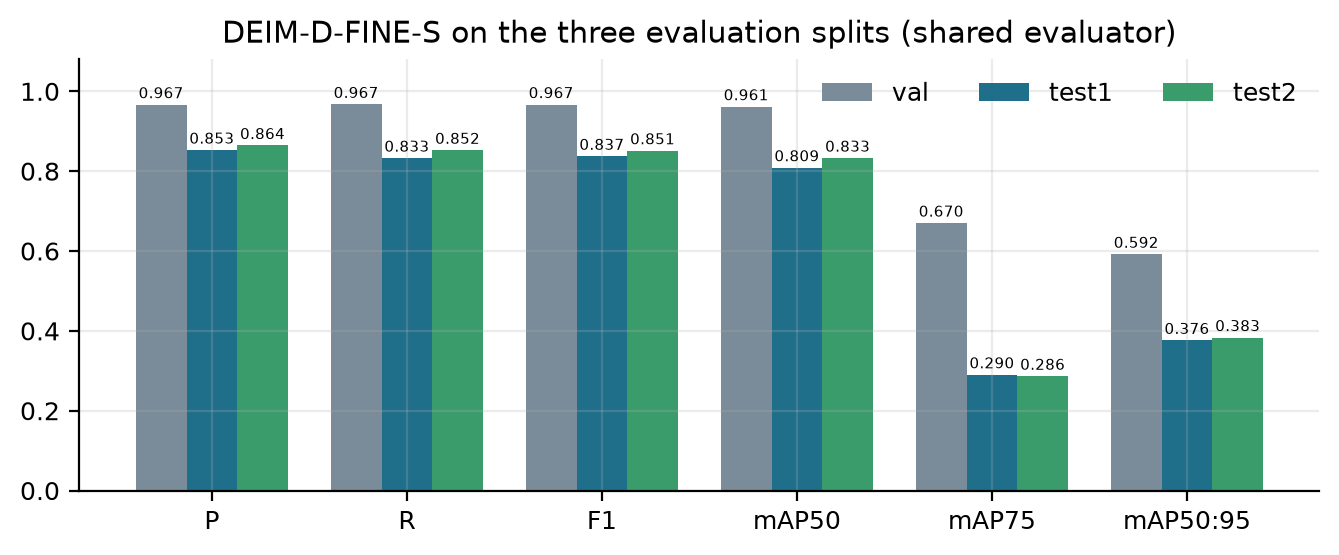
\includegraphics[width=0.9\linewidth]{figures/fig_split_comparison.png}
\caption{Validation versus held-out performance.}
\end{figure}

\begin{writehere}
Points to cover (Table~\ref{tab:compare}): best mAP50:95 and mAP75 of the three models on both test sets (mAP75 +0.029 / +0.040 over RF-DETR, +0.082 / +0.082 over YOLO26n); mAP50 and P slightly below RF-DETR on test1, mAP50 higher on test2; so the gain is in box precision, not in finding more objects; same val$\rightarrow$test drop as the other models; one seed only, so small differences ($<$0.01) are not conclusive yet.
\end{writehere}

\subsection{Per-class results}
\begin{table}[H]\centering
\caption{Per-class results on Test 1.}
\gentab{tab_per_class_test1}
\end{table}

\begin{table}[H]\centering
\caption{Per-class results on Test 2. Metal bucket has only 5 GT boxes.}
\gentab{tab_per_class_test2}
\end{table}

\begin{table}[H]\centering\small
\caption{Per-class AP50 on the test sets. YOLO26n: notebook (Ultralytics validator); RF-DETR-S and DEIM-D-FINE-S: shared evaluator. Best per class and split in bold.}
\resizebox{\linewidth}{!}{\gentab{tab_per_class_cmp_ap50}}
\end{table}

\begin{table}[H]\centering\small
\caption{Per-class AP50:95 on the test sets, same models.}
\resizebox{\linewidth}{!}{\gentab{tab_per_class_cmp_ap5095}}
\end{table}

\begin{figure}[H]\centering
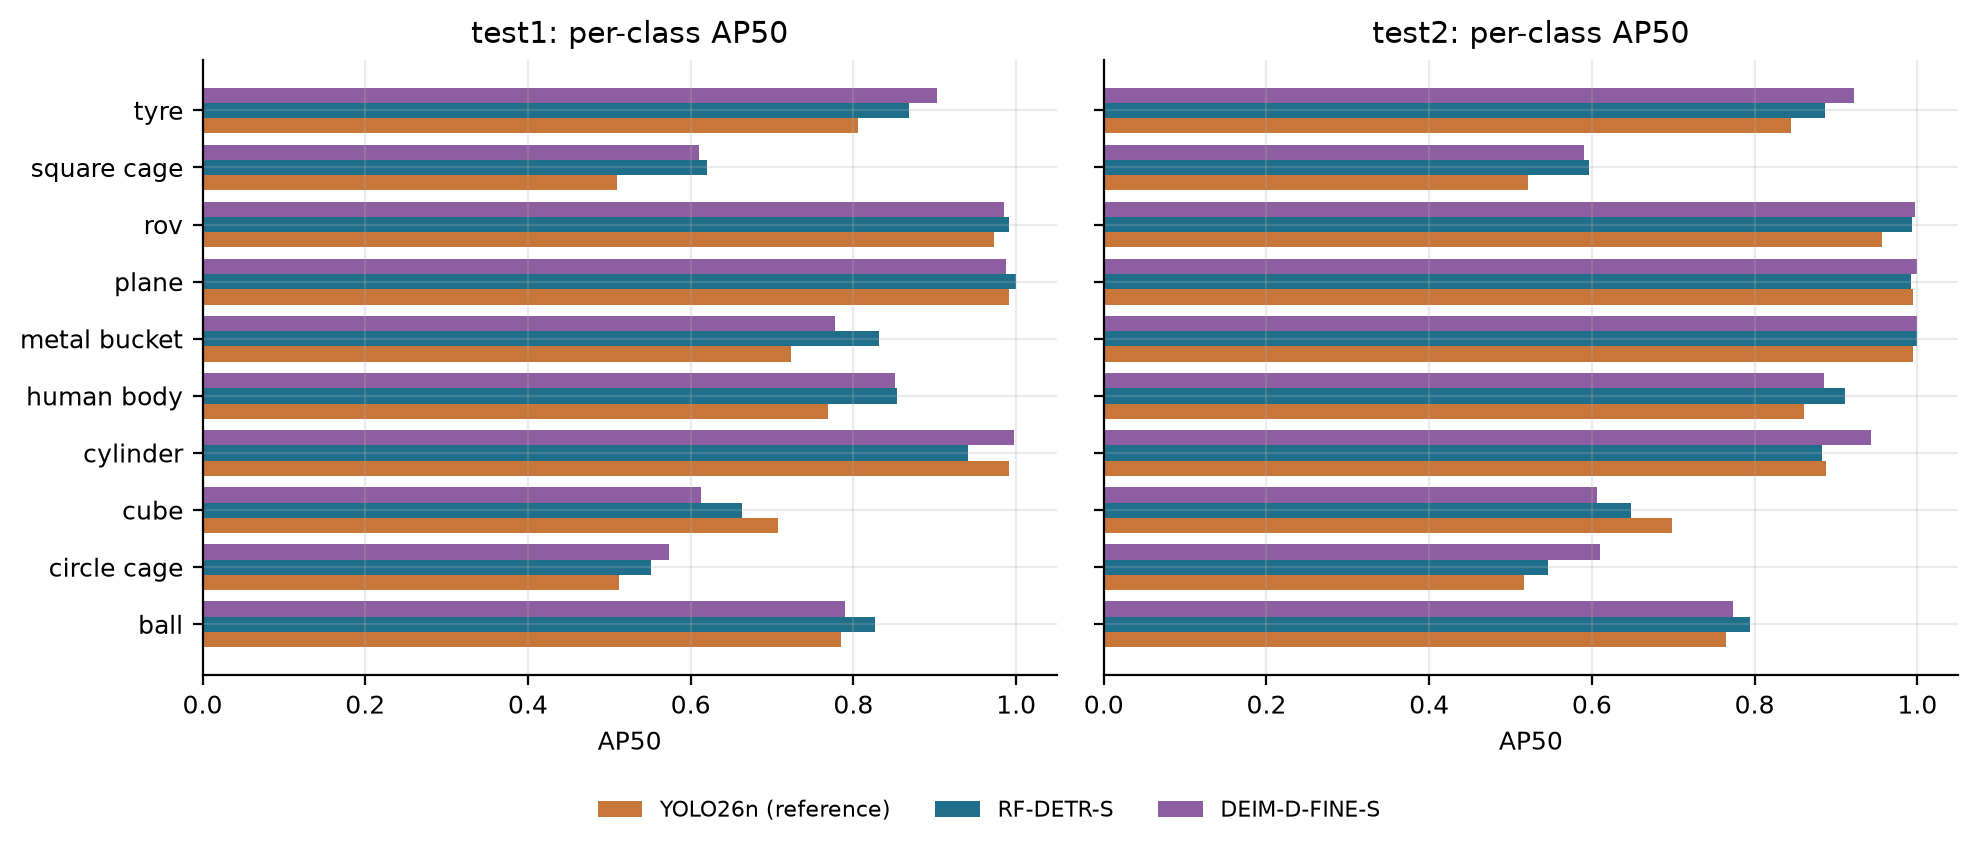
\includegraphics[width=\linewidth]{figures/fig_per_class_compare.png}
\caption{Per-class AP50 on Test 1 and Test 2 for the three models.}
\end{figure}

\begin{writehere}
Points to cover: DEIM has the best AP50:95 on 8 of 10 classes in test1 and 9 of 10 in test2; circle cage improves most at AP50 (0.573 / 0.609 vs 0.551 / 0.546 for RF-DETR); cube is the clear exception, lowest of the three models (AP50 0.612 / 0.606 vs YOLO26n 0.708 / 0.699); square cage about equal to RF-DETR; metal bucket has 6 / 5 test boxes, so its AP is unreliable.
\end{writehere}

\subsection{Precision--recall curves}
\begin{figure}[H]\centering
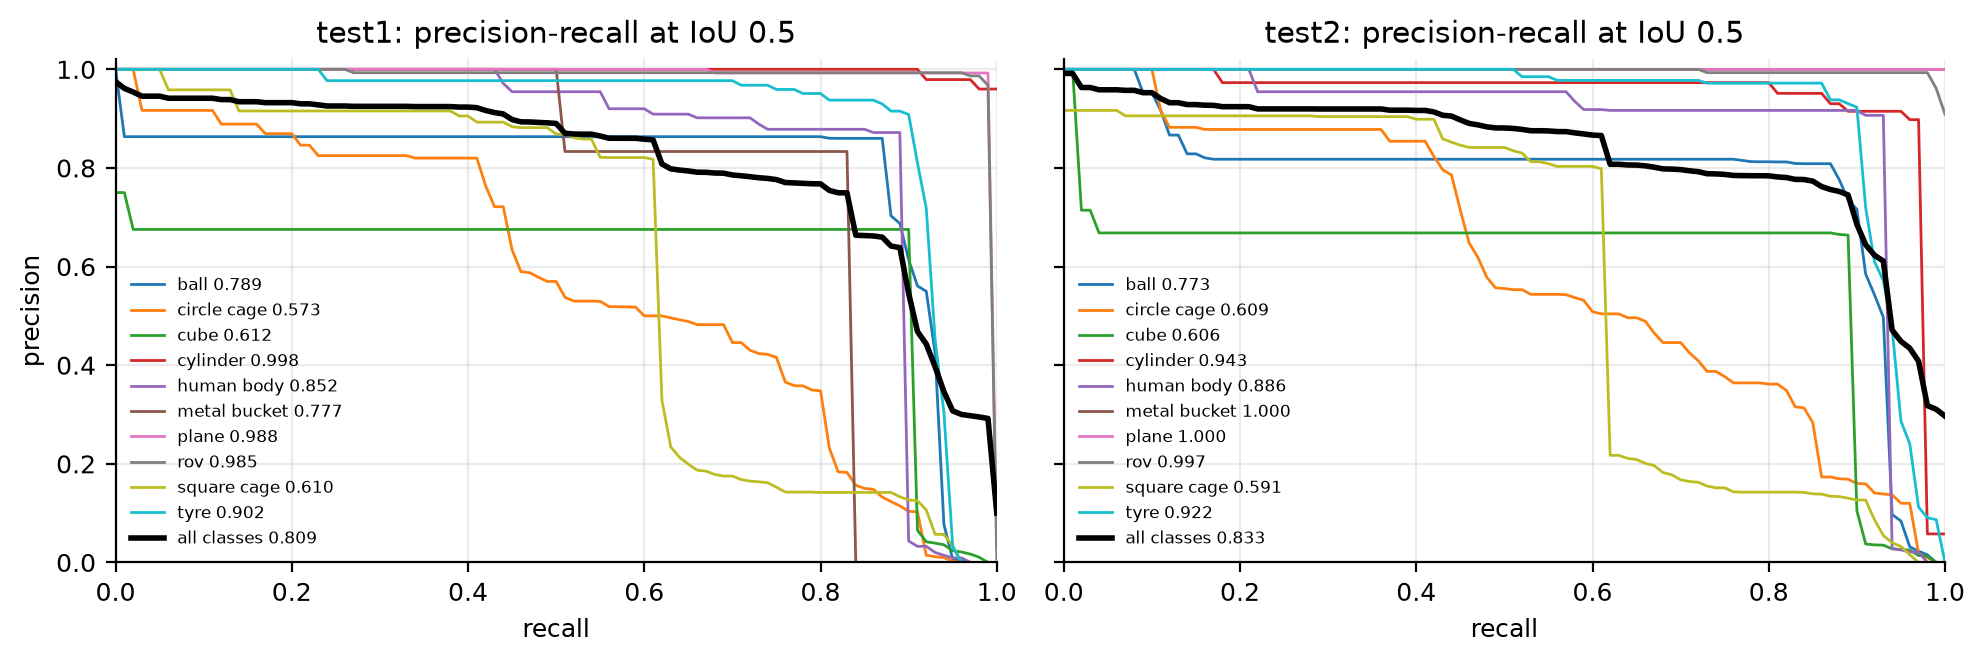
\includegraphics[width=\linewidth]{figures/fig_pr_curves.png}
\caption{Per-class precision--recall curves at IoU 0.5 (pycocotools, all areas). Legend values are AP50.}
\end{figure}

\subsection{Confusion between classes}
\begin{figure}[H]\centering
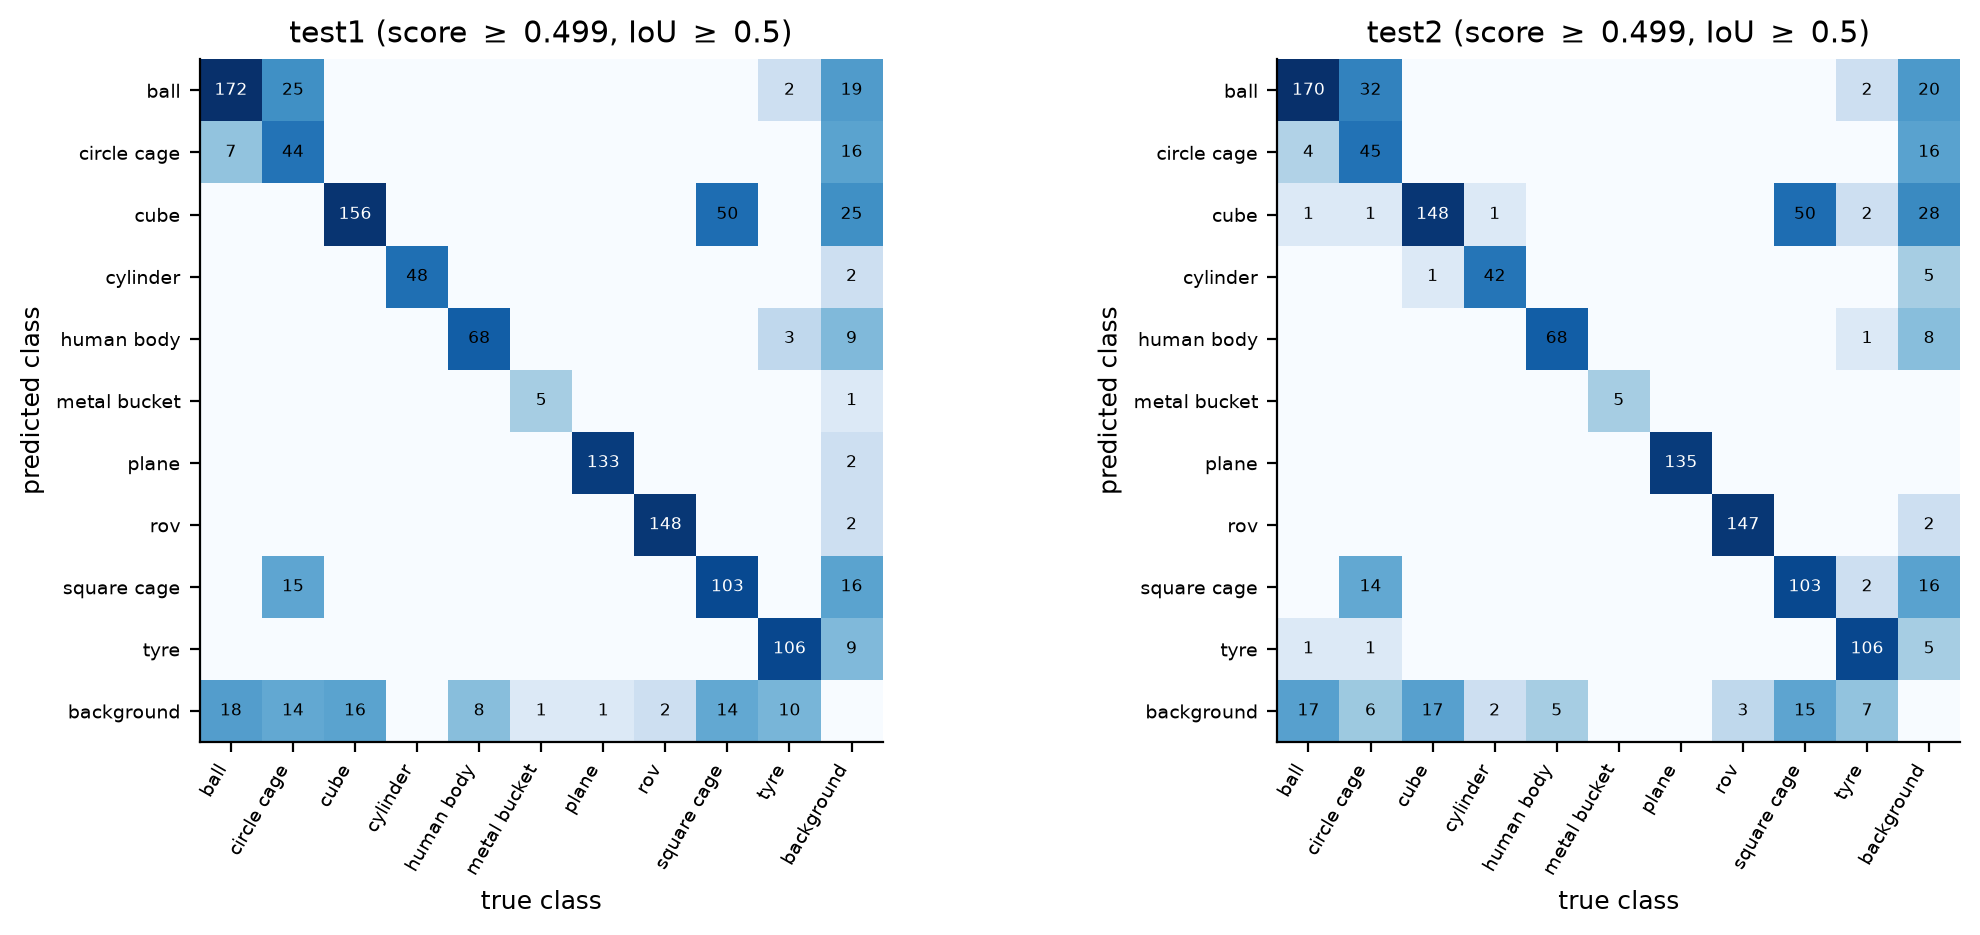
\includegraphics[width=\linewidth]{figures/fig_confusion_test.png}
\caption{Confusion matrices on the test sets. Detections with score $\geq$ 0.499 (the max-F1 confidence chosen on \emph{validation}), class-agnostic one-to-one matching at IoU $\geq$ 0.5. Rows: predicted class; columns: true class; ``background'' = unmatched.}
\end{figure}

\begin{writehere}
Points to cover: square cage predicted as cube 50 times in each test set, the same as RF-DETR (51 / 49), so this confusion is shared by both DETRs and explains cube's low precision; circle cage predicted as ball more often than with RF-DETR (25 / 32 vs 20 / 20) and as square cage 15 / 14; missed objects 84 / 72, unmatched detections 101 / 100 (RF-DETR: 80 / 76 and 76 / 86).
\end{writehere}

\subsection{Size-stratified results}
\begin{table}[H]\centering
\caption{DEIM-D-FINE-S AP on the UATD-relative size bins (tiny = area $\leq$ 2300\,px$^2$).}
\resizebox{\linewidth}{!}{\gentab{tab_size_bins}}
\end{table}

\begin{table}[H]\centering
\caption{Tiny versus non-tiny AP50:95 on the test sets, our two models (the YOLO26n notebook has no size bins). Best per column in bold.}
\gentab{tab_size_cmp}
\end{table}

\begin{figure}[H]\centering
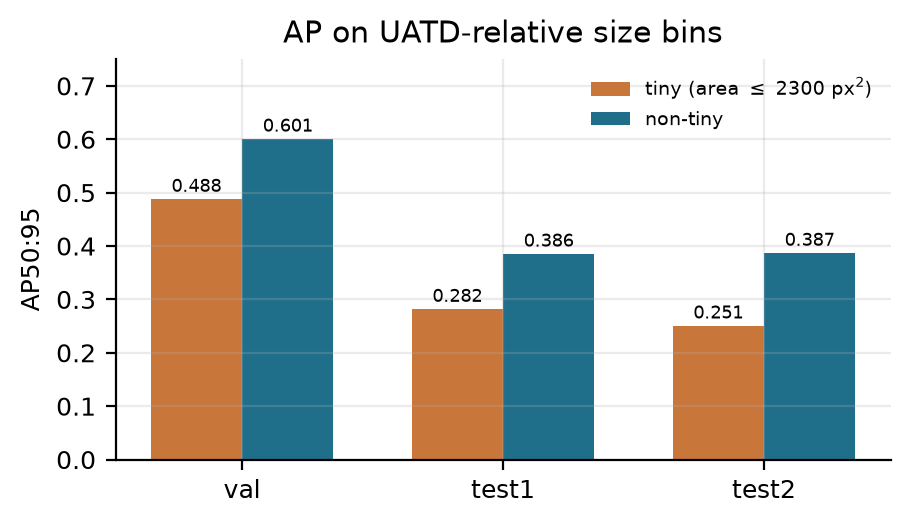
\includegraphics[width=0.6\linewidth]{figures/fig_size_bins.png}
\caption{DEIM-D-FINE-S tiny versus non-tiny AP50:95.}
\end{figure}

\begin{table}[H]\centering
\caption{Complete COCO-style statistics (pycocotools).}
\gentab{tab_coco_detail}
\end{table}

\begin{writehere}
Points to cover: DEIM is better on non-tiny boxes (0.386 / 0.387 vs 0.375 / 0.365) but worse on tiny boxes, clearly on test1 (0.282 vs 0.323) and slightly on test2 (0.251 vs 0.259); so its overall gain comes from larger objects; tiny objects remain the open problem for both, which supports the tiny-object track (roadmap step 8); possible factor to check later: Mosaic shrinks objects during training (320\,px tiles).
\end{writehere}

\subsection{Qualitative results}
\begin{figure}[H]\centering
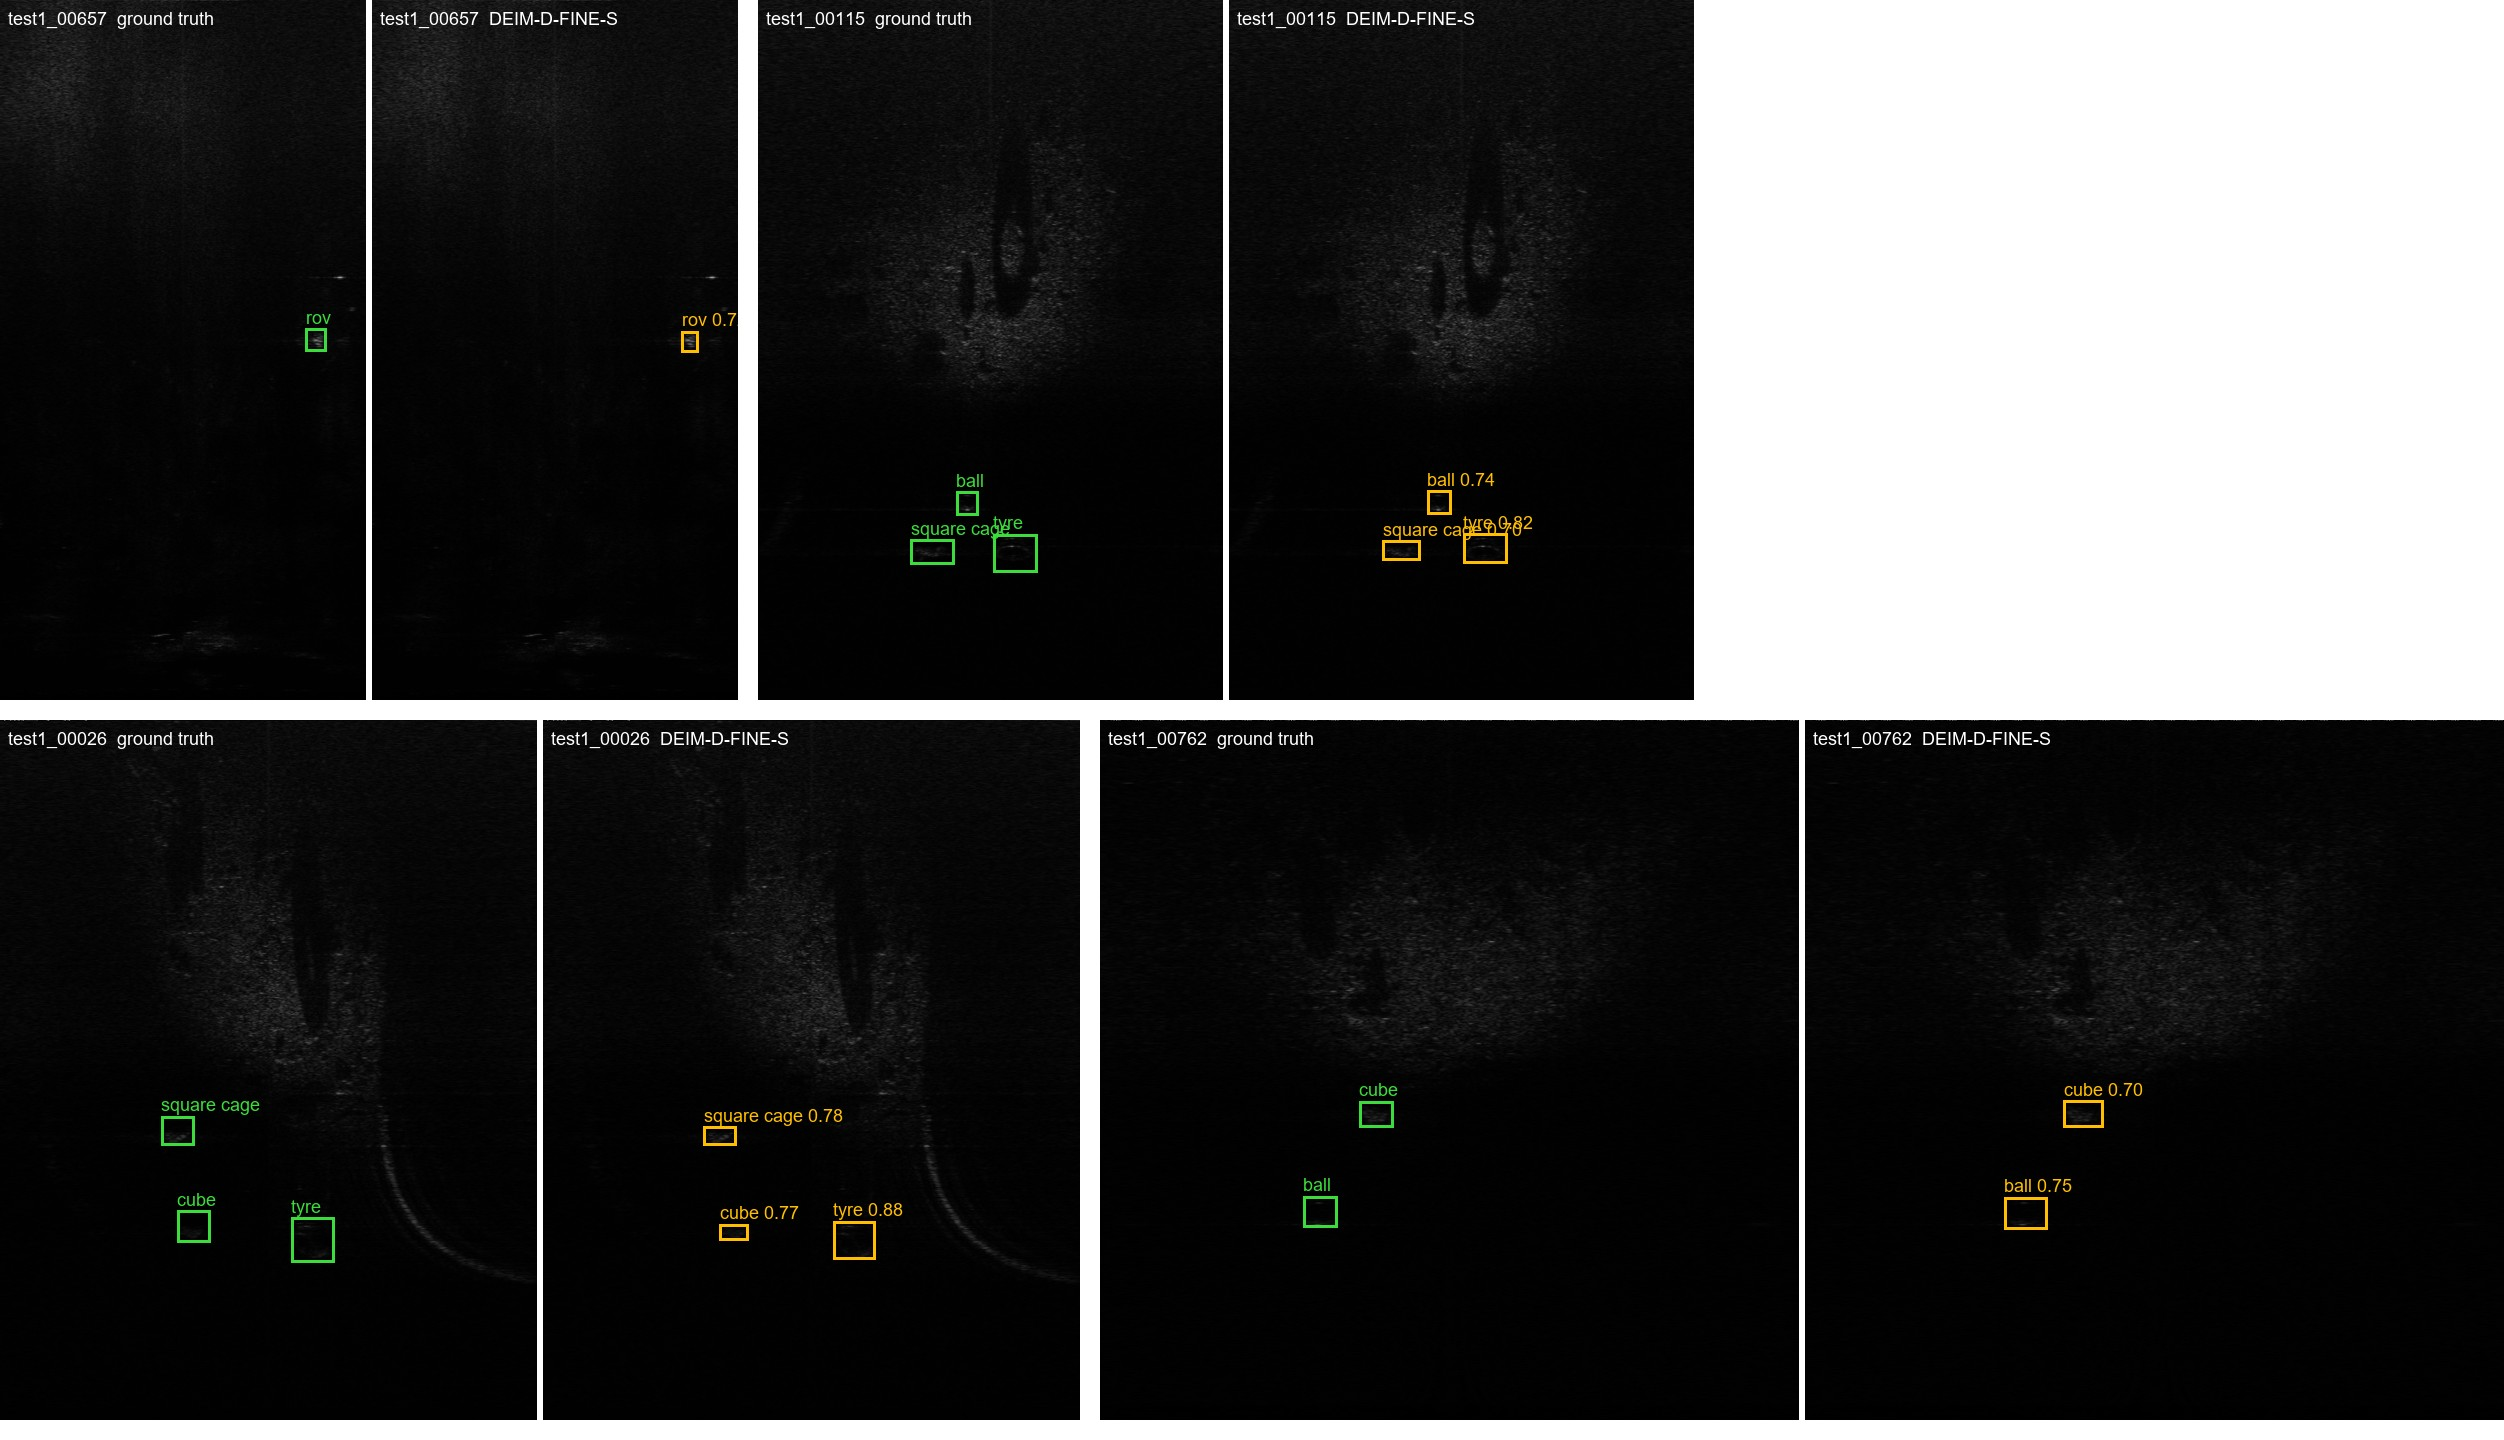
\includegraphics[width=\linewidth]{figures/fig_gallery_test1.jpg}
\caption{Test 1 examples (same 4 images as in the RF-DETR report, seed 42). Green: ground truth. Yellow: DEIM-D-FINE-S detections with score $\geq$ 0.499. Images are shown without contrast change.}
\end{figure}

\begin{figure}[H]\centering
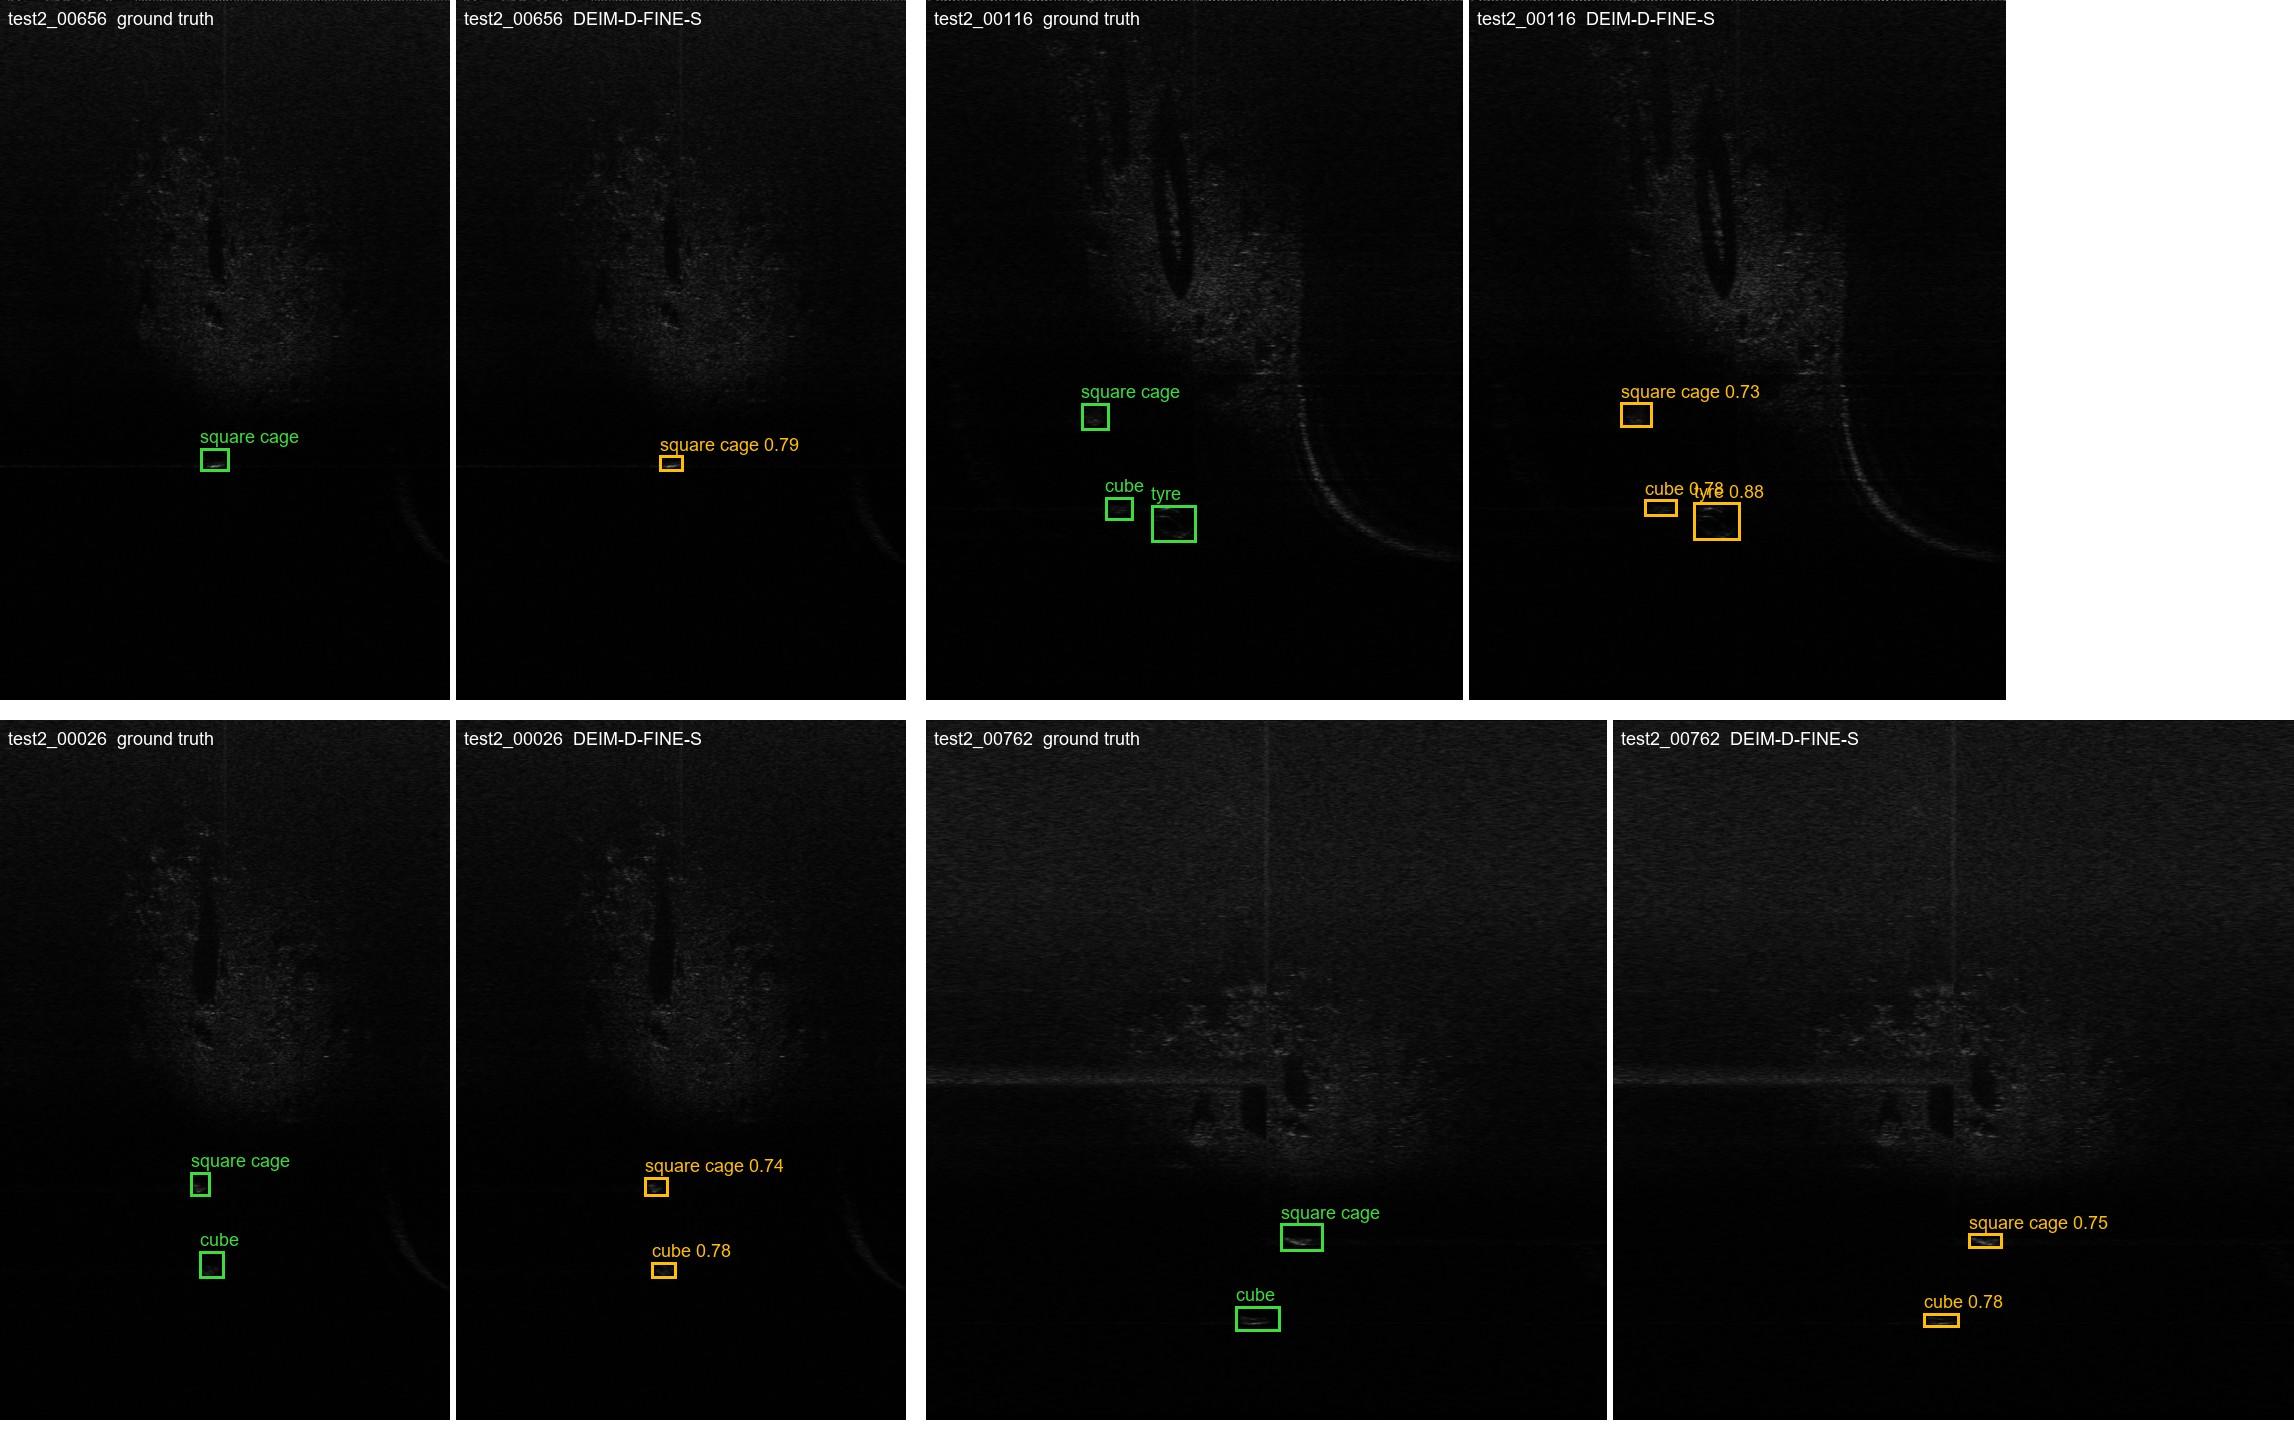
\includegraphics[width=\linewidth]{figures/fig_gallery_test2.jpg}
\caption{Test 2 examples (4 images, seed 42), same convention.}
\end{figure}

% ------------------------------------------------------------------ 6 efficiency
\section{Efficiency}\label{sec:eff}
\begin{table}[H]\centering
\caption{Model complexity and latency. GFLOPs and latency are roadmap step 4 and not measured yet.}
\begin{tabular}{lrrrrr}
\toprule
Model & Input & Params (M) & GFLOPs & T4 FP16 (ms) & T4 FP32 (ms)\\
\midrule
YOLO26n$^\dagger$ & 640 & 2.51 & 5.9 & -- & --\\
RF-DETR-S & 512 & pending & pending & pending & pending\\
DEIM-D-FINE-S & 640 & 10.23 & pending & pending & pending\\
\bottomrule
\end{tabular}\\[2pt]
{\footnotesize $^\dagger$From the notebook's training model summary. DEIM parameter count from its training log.}
\end{table}

% ------------------------------------------------------------------ 7 discussion
\section{Discussion}
\subsection{What the comparison shows}
\begin{writehere}
Your interpretation of the comparison above.
\end{writehere}
\subsection{Limitations}
\begin{writehere}
Points to cover: one seed per model; different input sizes (512 vs 640) and training recipes, each the model's own; DEIM is a comparison row only (RT-DETR lineage); YOLO26n numbers from Ultralytics' validator, not re-scored with our evaluator; efficiency not measured yet; val shares recording sessions with train, so val is optimistic.
\end{writehere}
\subsection{Next steps}
\begin{table}[H]\centering
\caption{Planned work (CLAUDE.md roadmap).}
\begin{tabular}{p{4.2cm}p{9.8cm}}
\toprule
Step & Work\\
\midrule
4 Efficiency & params, GFLOPs, batch-1 T4 latency (FP16 / FP32) for every model\\
5 Main pipeline & RF-DETR-N; RF-DETR at higher input resolution\\
6 Baselines & YOLOv12-n/s, FBRT-YOLO, Dome-DETR on the same split and evaluator\\
7 Error analysis & square cage $\rightarrow$ cube confusion (both DETRs), tiny-box recall, mAP50--mAP75 gap\\
8 Method & one tiny-object idea from an eligible venue on top of RF-DETR, with ablations\\
9 Final runs & 3 seeds for main models, final tables and figures\\
\bottomrule
\end{tabular}
\end{table}

% ------------------------------------------------------------------ appendix
\appendix
\section{Epoch log}\label{app:epochs}
\def\epochheader{Epoch & Loss & MAL & L1 & GIoU & FGL & mAP50:95 & mAP50 & mAP75 & AR100}

{\small
\setlength{\tabcolsep}{4pt}
\begin{longtable}{rrrrrrrrrr}
\caption{Per-epoch training losses (final decoder layer) and validation metrics (DEIM built-in evaluator, EMA weights).}\\
\toprule
\epochheader\\
\midrule
\endfirsthead
\toprule
\epochheader\\
\midrule
\endhead
\bottomrule
\endfoot
1 & 31.165 & 1.322 & 0.3970 & 1.037 & 1.004 & 0.409 & 0.793 & 0.357 & 0.659 \\
2 & 20.411 & 0.783 & 0.0963 & 0.482 & 1.232 & 0.491 & 0.903 & 0.452 & 0.684 \\
3 & 18.930 & 0.694 & 0.0913 & 0.457 & 1.226 & 0.508 & 0.921 & 0.483 & 0.693 \\
4 & 18.291 & 0.666 & 0.0871 & 0.438 & 1.222 & 0.522 & 0.935 & 0.518 & 0.703 \\
5 & 22.798 & 0.930 & 0.1270 & 0.842 & 1.088 & 0.523 & 0.934 & 0.517 & 0.683 \\
6 & 21.572 & 0.862 & 0.1017 & 0.736 & 1.129 & 0.518 & 0.929 & 0.499 & 0.666 \\
7 & 21.095 & 0.831 & 0.0940 & 0.698 & 1.143 & 0.518 & 0.933 & 0.503 & 0.656 \\
8 & 20.750 & 0.809 & 0.0870 & 0.676 & 1.151 & 0.520 & 0.937 & 0.509 & 0.645 \\
9 & 20.681 & 0.796 & 0.0899 & 0.686 & 1.141 & 0.519 & 0.938 & 0.507 & 0.645 \\
10 & 20.350 & 0.787 & 0.0804 & 0.648 & 1.157 & 0.520 & 0.941 & 0.507 & 0.642 \\
11 & 20.257 & 0.783 & 0.0806 & 0.645 & 1.158 & 0.522 & 0.941 & 0.514 & 0.648 \\
12 & 20.069 & 0.767 & 0.0798 & 0.631 & 1.162 & 0.523 & 0.940 & 0.517 & 0.649 \\
13 & 20.061 & 0.772 & 0.0789 & 0.633 & 1.159 & 0.525 & 0.942 & 0.522 & 0.653 \\
14 & 19.844 & 0.760 & 0.0740 & 0.616 & 1.166 & 0.527 & 0.939 & 0.527 & 0.658 \\
15 & 19.840 & 0.759 & 0.0764 & 0.620 & 1.162 & 0.528 & 0.943 & 0.525 & 0.658 \\
16 & 19.657 & 0.747 & 0.0728 & 0.605 & 1.167 & 0.530 & 0.945 & 0.525 & 0.656 \\
17 & 19.553 & 0.745 & 0.0714 & 0.593 & 1.172 & 0.531 & 0.948 & 0.525 & 0.659 \\
18 & 19.528 & 0.735 & 0.0719 & 0.600 & 1.167 & 0.531 & 0.949 & 0.532 & 0.661 \\
19 & 19.493 & 0.738 & 0.0711 & 0.591 & 1.170 & 0.534 & 0.948 & 0.540 & 0.662 \\
20 & 19.461 & 0.736 & 0.0720 & 0.594 & 1.167 & 0.537 & 0.950 & 0.542 & 0.664 \\
21 & 19.461 & 0.739 & 0.0711 & 0.596 & 1.166 & 0.538 & 0.951 & 0.543 & 0.667 \\
22 & 19.354 & 0.731 & 0.0692 & 0.588 & 1.170 & 0.539 & 0.950 & 0.552 & 0.669 \\
23 & 19.336 & 0.732 & 0.0698 & 0.583 & 1.170 & 0.540 & 0.951 & 0.558 & 0.668 \\
24 & 19.347 & 0.735 & 0.0703 & 0.584 & 1.169 & 0.544 & 0.956 & 0.556 & 0.669 \\
25 & 19.192 & 0.728 & 0.0677 & 0.572 & 1.174 & 0.547 & 0.956 & 0.570 & 0.665 \\
26 & 19.105 & 0.723 & 0.0663 & 0.565 & 1.173 & 0.546 & 0.951 & 0.569 & 0.662 \\
27 & 19.140 & 0.724 & 0.0676 & 0.570 & 1.171 & 0.549 & 0.953 & 0.581 & 0.663 \\
28 & 19.166 & 0.724 & 0.0673 & 0.567 & 1.172 & 0.549 & 0.952 & 0.576 & 0.662 \\
29 & 19.062 & 0.714 & 0.0664 & 0.569 & 1.169 & 0.550 & 0.952 & 0.579 & 0.663 \\
30 & 19.024 & 0.714 & 0.0654 & 0.562 & 1.173 & 0.554 & 0.953 & 0.590 & 0.666 \\
31 & 18.985 & 0.713 & 0.0658 & 0.561 & 1.171 & 0.554 & 0.952 & 0.595 & 0.670 \\
32 & 19.043 & 0.719 & 0.0663 & 0.563 & 1.173 & 0.556 & 0.955 & 0.601 & 0.672 \\
33 & 18.914 & 0.712 & 0.0644 & 0.556 & 1.174 & 0.558 & 0.955 & 0.611 & 0.670 \\
34 & 18.958 & 0.715 & 0.0645 & 0.557 & 1.175 & 0.557 & 0.958 & 0.599 & 0.668 \\
35 & 18.149 & 0.665 & 0.0783 & 0.456 & 1.219 & 0.563 & 0.958 & 0.616 & 0.684 \\
36 & 17.907 & 0.653 & 0.0764 & 0.446 & 1.216 & 0.565 & 0.957 & 0.615 & 0.693 \\
37 & 17.772 & 0.644 & 0.0748 & 0.439 & 1.216 & 0.569 & 0.957 & 0.610 & 0.703 \\
38 & 17.685 & 0.641 & 0.0734 & 0.437 & 1.214 & 0.573 & 0.959 & 0.618 & 0.709 \\
39 & 17.572 & 0.634 & 0.0726 & 0.430 & 1.216 & 0.575 & 0.958 & 0.621 & 0.711 \\
40 & 17.600 & 0.636 & 0.0728 & 0.433 & 1.213 & 0.576 & 0.959 & 0.628 & 0.713 \\
41 & 17.488 & 0.633 & 0.0713 & 0.425 & 1.212 & 0.576 & 0.958 & 0.625 & 0.716 \\
42 & 17.490 & 0.632 & 0.0725 & 0.425 & 1.212 & 0.579 & 0.961 & 0.632 & 0.719 \\
43 & 17.360 & 0.628 & 0.0687 & 0.420 & 1.211 & 0.580 & 0.961 & 0.631 & 0.720 \\
44 & 17.336 & 0.626 & 0.0688 & 0.419 & 1.209 & 0.581 & 0.960 & 0.636 & 0.721 \\
45 & 17.295 & 0.623 & 0.0689 & 0.419 & 1.209 & 0.582 & 0.960 & 0.634 & 0.723 \\
46 & 17.233 & 0.620 & 0.0674 & 0.415 & 1.210 & 0.585 & 0.961 & 0.641 & 0.726 \\
47 & 17.235 & 0.621 & 0.0679 & 0.414 & 1.208 & 0.587 & 0.960 & 0.642 & 0.730 \\
48 & 17.176 & 0.616 & 0.0678 & 0.412 & 1.208 & 0.586 & 0.961 & 0.644 & 0.732 \\
49 & 17.120 & 0.615 & 0.0669 & 0.411 & 1.205 & 0.588 & 0.963 & 0.643 & 0.731 \\
50 & 17.051 & 0.611 & 0.0666 & 0.406 & 1.205 & 0.589 & 0.963 & 0.649 & 0.731 \\
51 & 17.034 & 0.613 & 0.0660 & 0.403 & 1.206 & 0.589 & 0.960 & 0.652 & 0.734 \\
52 & 17.038 & 0.613 & 0.0663 & 0.402 & 1.205 & 0.590 & 0.963 & 0.650 & 0.735 \\
53 & 16.994 & 0.610 & 0.0658 & 0.402 & 1.204 & 0.590 & 0.962 & 0.659 & 0.732 \\
54 & 16.950 & 0.609 & 0.0661 & 0.400 & 1.202 & 0.590 & 0.962 & 0.651 & 0.735 \\
55 & 16.931 & 0.608 & 0.0653 & 0.398 & 1.203 & 0.590 & 0.961 & 0.652 & 0.736 \\
56 & 16.914 & 0.605 & 0.0653 & 0.398 & 1.202 & 0.589 & 0.961 & 0.666 & 0.738 \\
57 & 16.855 & 0.604 & 0.0651 & 0.396 & 1.200 & 0.589 & 0.960 & 0.668 & 0.740 \\
58 & 16.834 & 0.602 & 0.0644 & 0.394 & 1.202 & 0.591 & 0.960 & 0.667 & 0.739 \\
59 & 16.182 & 0.572 & 0.0668 & 0.357 & 1.190 & 0.592 & 0.961 & 0.670 & 0.738 \\
60 & 15.952 & 0.563 & 0.0637 & 0.345 & 1.185 & 0.590 & 0.962 & 0.675 & 0.736 \\

\end{longtable}
}

\section{Reproducibility}
\begin{table}[H]\centering
\caption{Where everything lives in the repository.}
\begin{tabular}{p{5cm}p{9cm}}
\toprule
Item & Location\\
\midrule
Code & \url{https://github.com/azmineamin/uatd-sonar-detection}\\
DEIM config & \texttt{configs/deim/uatd\_deim\_dfine\_s.yml}\\
Training & \texttt{scripts/train\_deim.py}, \texttt{notebooks/kaggle\_deim.ipynb}\\
Prediction + selection & \texttt{scripts/predict\_deim.py} (\texttt{selection.json})\\
Shared evaluator & \texttt{src/uatd/eval\_coco.py}\\
Run files & \texttt{results/deim/dfine\_s\_s0/}\\
This report's assets & \texttt{scripts/make\_report\_assets.py --model deim}\\
\bottomrule
\end{tabular}
\end{table}

\end{document}
